% 1988 年广东卷理工农医类第二卷第二题：四棱锥 P-ABCD
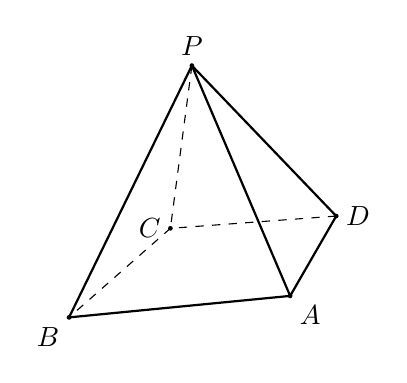
\begin{tikzpicture}[scale=0.78,>=stealth]
  \coordinate (P) at (2.0,4.1);
  \coordinate (B) at (0,0);
  \coordinate (A) at (3.6,0.35);
  \coordinate (D) at (4.35,1.65);
  \coordinate (C) at (1.65,1.45);
  \draw[thick] (P)--(B) (P)--(A) (P)--(D);
  \draw[dashed] (P)--(C);
  \draw[thick] (B)--(A)--(D);
  \draw[dashed] (D)--(C)--(B);
  \fill (P) circle (1.1pt) node[above] {$P$};
  \fill (A) circle (1.1pt) node[below right] {$A$};
  \fill (B) circle (1.1pt) node[below left] {$B$};
  \fill (C) circle (1.1pt) node[left] {$C$};
  \fill (D) circle (1.1pt) node[right] {$D$};
\end{tikzpicture}
